%update: Dec 02 figures inserted
%update: Nov 29 citation done, bug fixes
%update: Nov 25 draft

\begin{savequote}[75mm] 
We see the world, not as it is, but as we are, or, as we are conditioned to see it.
\qauthor{Stephen R. Covey} 
\end{savequote}

\chapter{Statistically photoresponse analyzing of CdS nanowires by \emph{in situ} TEM}

\newthought{To find clues for flexible optoelectronics}, light, force and electrons are all important factors to be considered. I demonstrate that high resolution transmission electron microscopy (HRTEM) paired with light illumination of a sample and its electrical probing can be utilized for the in situ study of initiated photocurrents in free-standing nanowires. Morphology, phase and crystallographic information from numerous individual CdS nanowires is obtained simultaneously with photocurrent measurements. Our results indicate that elastically bent (perpendicular to z-axis) CdS nanowires possessing a wurtzite structure show statistically unchanged values of ON/OFF (photocurrent/dark current) ratios. Photocurrent spectroscopy reveals red shifts of several nanometers in the cut-off wavelength after nanowire bending. This results from deformation-induced defects, e.g. twins or stacking faults, as confirmed by HRTEM. The dark current and photocurrent stabilities of bent CdS nanowires make them promising candidates for future flexible electronics, optoelectronics and photovoltaics.\\

\section{Introduction}
Flexible electronics and optoelectronics have attracted considerable research interest in recent years due to the growing demand for lightweight electronic devices having high portability and low manufacturing cost, as compared to conventional bulk silicon technology.\cite{Boland2010,Liu2015,Long2012} With large surface-to-volume and aspect ratios, high carrier mobility, and easily chemically decorated surfaces which could further be modified and functionalized, one-dimensional inorganic semiconducting nanostructures have proven to be key candidates for future flexible displays,\cite{Klauk2008} lithium-ion batteries,\cite{Wang2015}, supercapacitors,\cite{Li2014} solar cells,\cite{Zhang2012} generators,\cite{Fan2012} sensors,\cite{Zhang2014c} etc. One of the main existing challenges for such applications is the nanostructures electrical and mechanical operational stabilities. Even though some reports claimed that the nanowire conductivity is unchanged during mechanical deformations, there have been no in-depth investigations concerning the photoconductivity or photocurrent spectroscopy of individual nanowires under conditions which would allow the direct visualization of deformation-induced defects. Thus it is still unclear how the atomic structure changes in deformed nanowires affect their photoresponse. It is noteworthy that the latter was assumed to be unstable during elastic deformations.\cite{Antsov2014}
Here, we thoroughly address these issues by performing pioneering in situ HRTEM experiments using a specially designed optical TEM holder. We chose cadmium sulfide (CdS), a direct band gap semiconducting material widely used in diverse photoelectronic devices, as the test nanowire material.\cite{Xing2015} Using simultaneous electrical probing and HRTEM imaging, the currents induced in light-illuminated samples were measured by a source-measuring unit coupled with a light source, while at the same time allowing detailed visualization of bending deformation features. \\
The first part of our results establishes a relationship between bending deformations and current values. In order to exclude the uncertainty introduced by the contact geometry (which is also an important factor for future flexible devices), and in order to account for the morphological diversity of the nanowires, we performed a careful statistical analysis of numerous sets of experimental runs. The second part of the work relies on photocurrent spectroscopy measurements, which showed red-shifts for the cut-off wavelength of the deformed nanowires that were considered to be a result of deformation-induced defects. The third and final part of the work attempts to characterize these defects using HRTEM imaging. 

\section{Experimental}
CdS nanowires were synthesized via a chemical vapor deposition (CVD) method, as described in our earlier work.\cite{Zhang2015} The typical size of nanowires tested was about 100 nm in diameter and a few micrometers in length. The crystal structure of the nanowires is wurzite, as confirmed by X-ray diffraction and SAED pattern, which are presented in Figure \ref{fig:6_s1}. The samples were firmly attached to a freshly-cut flattened gold tip using a thin layer of an electrically-conductive silver epoxy. \\

\begin{figure}  
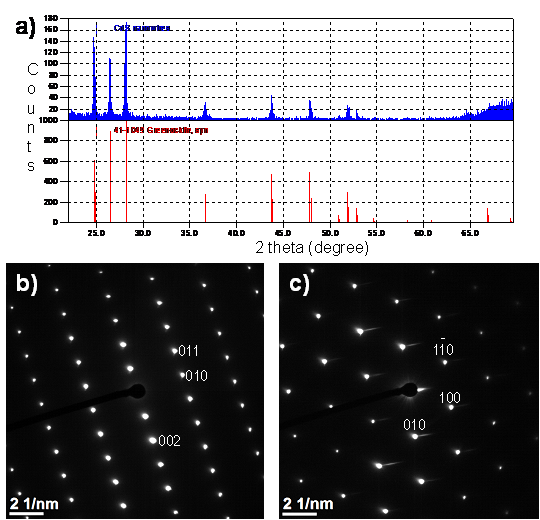
\includegraphics[width=\textwidth]{figures/figure6_s1}
\caption[CdS crystallography]
{(a) XRD data of the nanowire sample (upper panel) fits a CdS hexagonal phase, JCPDS Card No. 41-1049 (lower panel). (b,c) Two SAED patterns of a CdS nanowire taken along the [100] and [001] directions, respectively. 
\label{fig:6_s1}}
\end{figure}


As illustrated in Figure \ref{fig:6_1}, the system comprises an optical fiber-compatible TEM specimen holder, featuring a piezo-tube which allows for a metallic probe (connected to a sourcemeter) and multimode optical fiber (connected to a light source) to be precisely positioned inside the pole piece of the microscope. The probe (with a tip radius between 50 nm and several micrometers) was aligned with the center of the optical fiber (with a 200 um diameter core) at a distance of about 0.5 mm. Probing, mechanical manipulations, HRTEM imaging and selected area electron diffraction (SAED) studies were performed using an energy-filtering 300 kV JEM 3100FEF high-resolution TEM, under high vacuum (10-5 Pa) at room temperature. The specimen holder is an upgraded version of a piezo-driven optical TEM holder (Nanofactory Instruments AB).\\

\begin{figure}  
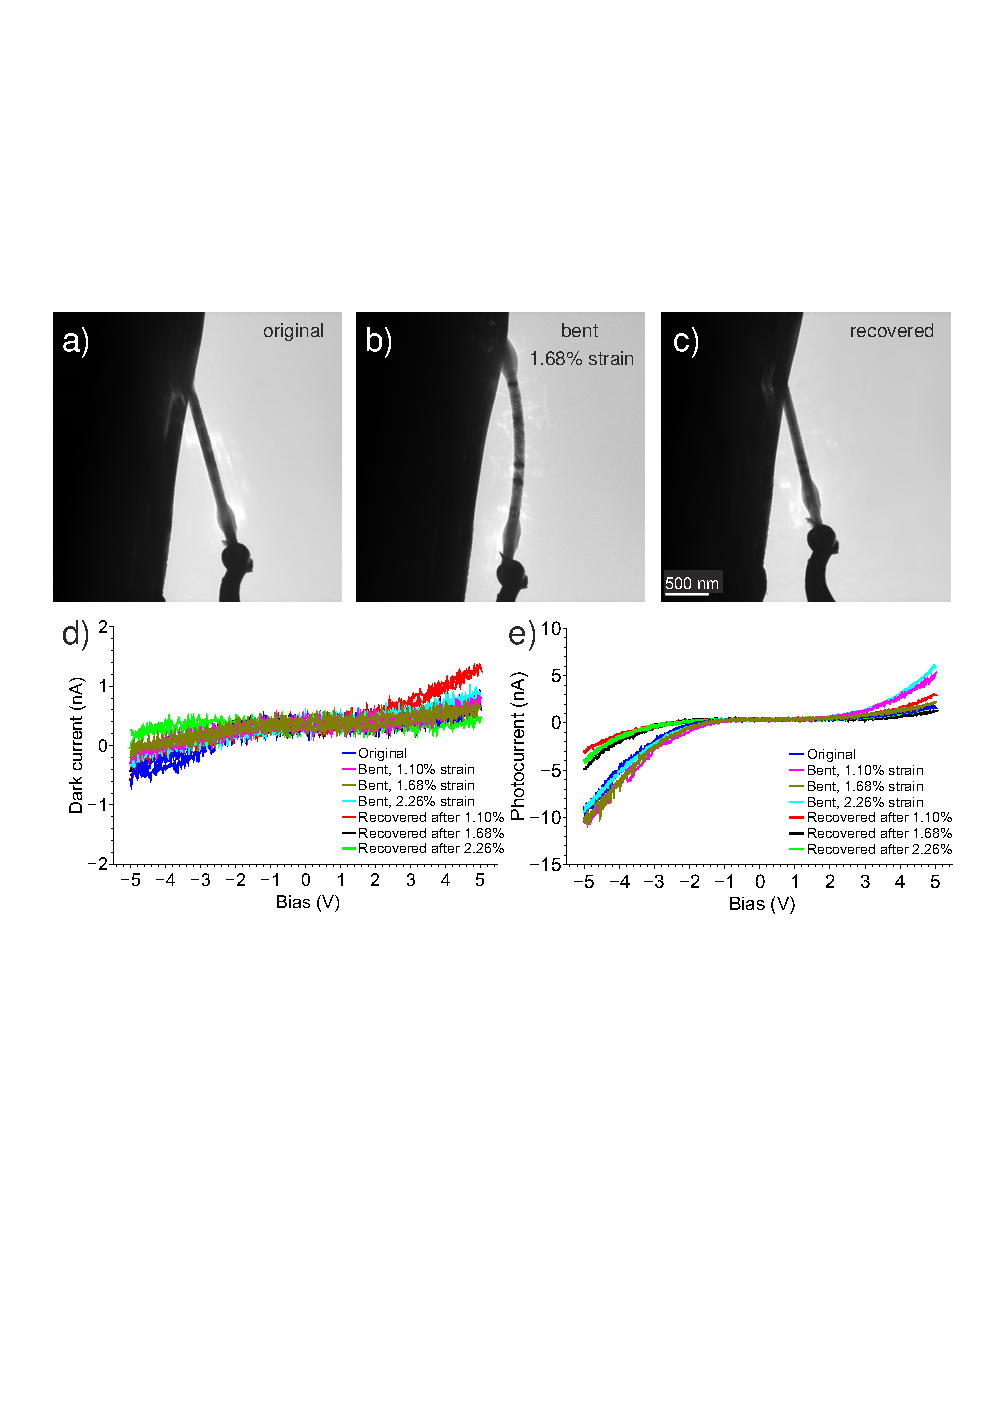
\includegraphics[width=\textwidth]{figures/figure6_2}
\caption[Deformation and I-V measurements]
{Representative TEM images of the original (a), bent (b) and recovered (c) states of an individual CdS nanowire positioned between fixed Au (left hand side) and movable W (right hand side) electrodes; and a summary of dark current (d) and photocurrent (e) measurements at different stages of the bending-recovery process. Calculated strains are marked on the TEM image and I-V plots. 
\label{fig:6_2}}
\end{figure}

Two types of in situ experiments were performed. Photocurrent I-V measurements, described in Figure \ref{fig:6_1} (Scheme 1), test the current-voltage response of nanowires which are illuminated using a laser diode with a working wavelength of 488 nm. Photocurrent spectroscopy measurements, described in Figure \ref{fig:6_1} (Scheme 2), test the wavelength dependency of the electrical current which is generated inside the nanowire under light irradiation. The light source for photocurrent spectroscopy was a laser driven white light source, monochromated in order to carry out wavelength-selected measurements. In order to improve the signal-to-noise (S/N) ratio, a chopper and a lock-in amplifier were introduced in the measurement system for this case. \\

\begin{figure}  
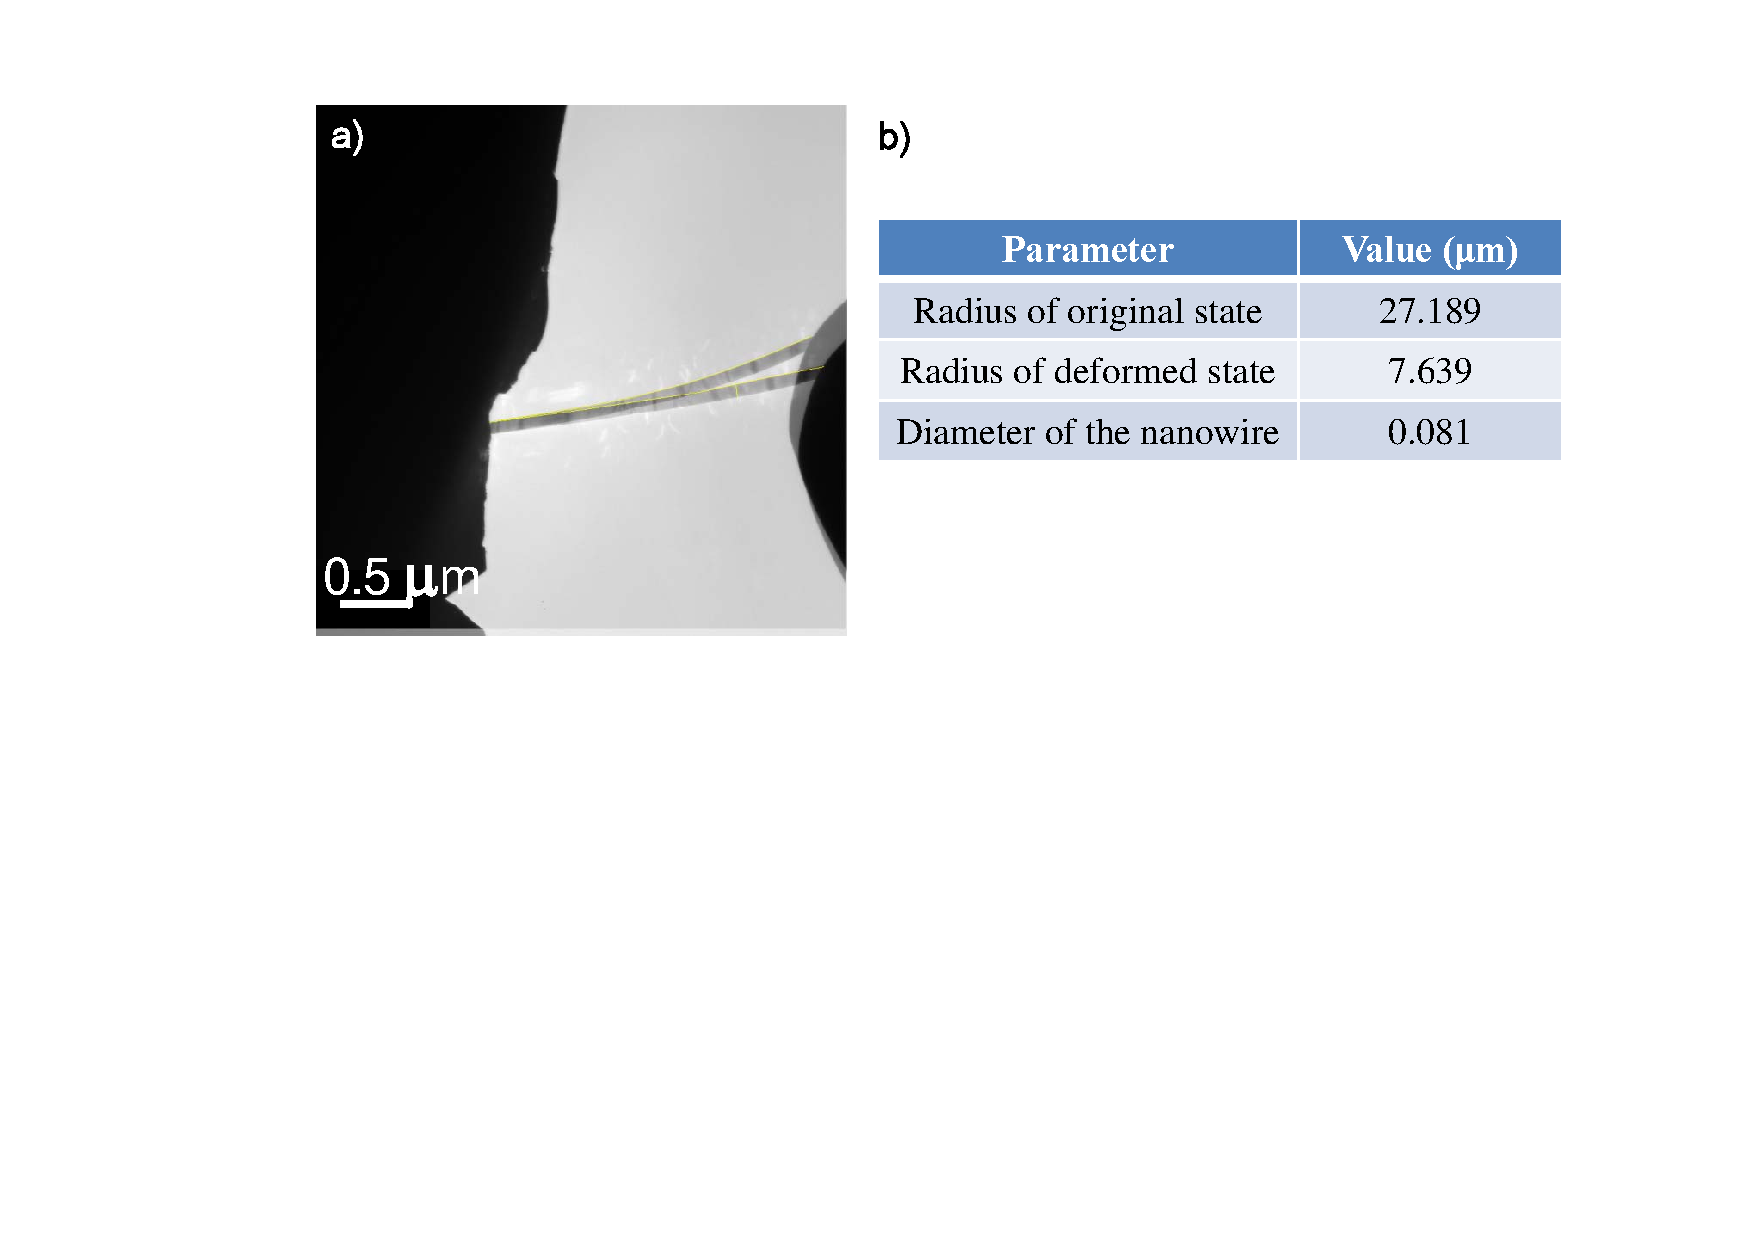
\includegraphics[width=130pt,angle=-90]{figures/figure6_s2}
\caption[Strain value]
{Strain measurements for an individual nanowire. (a) Two overlapped images of the nanowire, before and after deformation. (b) Measurements of the diameter of the nanowire, and its radius of curvature for the two cases. The strain was calculated as d/R, where d represents the diameter and R the radius. The values were measured using the {\em Digimizer} software.
\label{fig:6_s2}}
\end{figure}

\section{Results and Disscussions}
Dark currents and photocurrents of the nanowires were measured by the sourcemeter before bending deformation, during deformation and after complete nanostructure recovery. While the majority of nanowires revealed stable contact properties during the deformations and recoveries, some nanowires deviated from this behavior and showed increased or decreased currents. Figure \ref{fig:6_2}a illustrates a contact to a nanowire in its original non-deformed state. The average strain was defined as $\varepsilon = \frac{d}{R}$, where $d$ is a diameter of the nanowire and $R$ is its radius of curvature. These two parameters were measured by employing a curvature fit to the TEM images, as shown in Figure \ref{fig:6_s2} for a representative nanowire. In order to achieve a strong and stable physical contact, the probe was slightly pressed towards the nanowire, as shown in Figure \ref{fig:6_2}a. The probe was then moved left about 200 nm, resulting in a strain of up to 1.68\%, as shown in Figure \ref{fig:6_2}b. The nanowire was then recovered to its original state by retracting the probe, as shown in Figure \ref{fig:6_2}c. For each state, I-V measurements were performed in both dark and illuminated conditions, as summarized in Figure \ref{fig:6_2}d-e. In an attempt to get a better understanding of the relationship between the deformation states of the nanowires and their electrical and optical responses, numerous experiments were carried out for a comprehensive statistical analysis. The most important parameter is the light ON/OFF ratio (photocurrent to dark current ratio) of the nanowires. We define three ON/OFF ratios, corresponding to the original, deformed and recovered states as:\\
{\center
$R_{ori} = \frac{I_{ph-ori}}{I_{dr-ori}}$, $R_{def} = \frac{I_{ph-def}}{I_{dk-def}}$, $R_{rec} = \frac{I_{ph-rec}}{I_{dk-rec}}$\\}

, where $dk$ and $ph$ correspond to dark current and photocurrent, while $ori$, $def$ and $rec$ refer to the original, deformed and recovered states of the nanowire, respectively.\\

\begin{figure}  
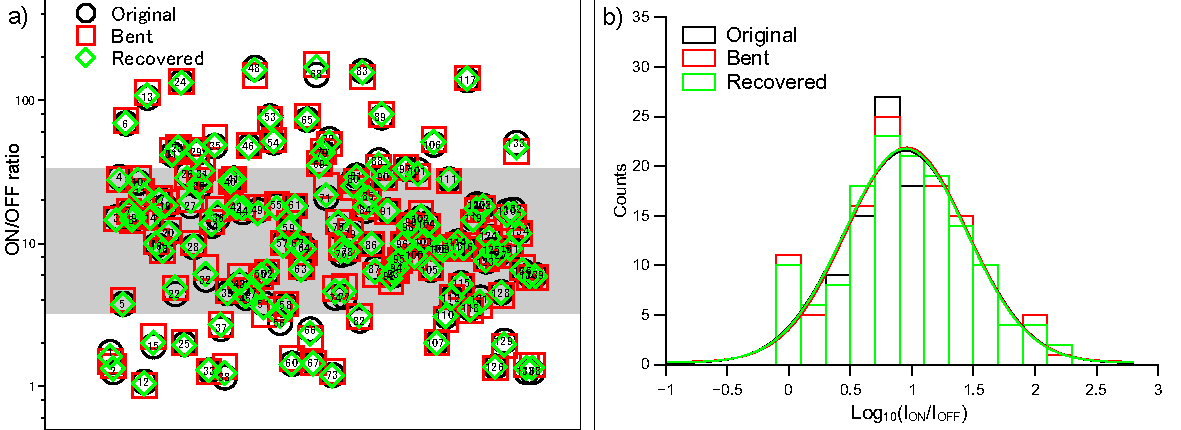
\includegraphics[width=\textwidth]{figures/figure6_3}
\caption[Statistical distribution of ON/OFF ratios]
{Statistical distribution of the measured ON/OFF (photocurrent/dark current) ratios for 139 bending/recovery experiments undertaken on individual CdS nanowires. (a) ON/OFF ratio scatter; a gray region, where the majority of cases were documented, is drawn as a guide to the eye. (b) Statistical analysis of the data in (a); the lines represent Gaussian fits to the 3 histograms.
\label{fig:6_3}}
\end{figure}

As shown in Figure \ref{fig:6_3}a, although the values vary from case to case, caused by probing-induced contact changes, the ON/OFF ratios are rather stable for each individual case. The statistical distribution of the ON/OFF values in Figure \ref{fig:6_3}b confirms this trend on a wider scale and also allows us to estimate an average value of around 10. The results of stable ON/OFF ratios were most common; however, some data showed deviations. The reason is the fact that our setup has limitations with respect to the number of electrodes employed. With only two electrodes, contact resistance becomes an important uncertainty.\cite{Hummelgard2011} The effects of this variable are however absorbed by our statistical analysis, where it is normally distributed. The independent nature of this variable with respect to the resistance of the nanowire itself allows their contributions to be separated, enabling us to observe the effects which are due to the intrinsic nature of our sample.

\begin{figure}  
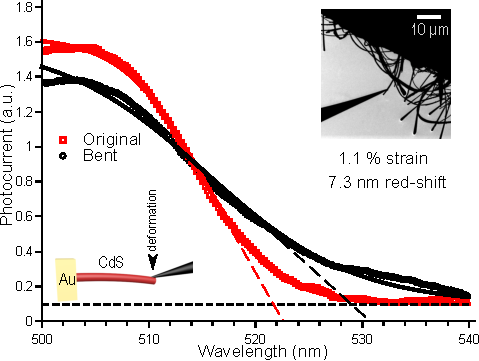
\includegraphics[width=250pt]{figures/figure6_4}
\caption[Photocurrent spectroscopy of deformed CdS NW]
{Photocurrent spectroscopy measurements performed on a representative individual CdS nanowire. The spectra have been fitted with logistic decay functions (solid lines); the regions of the curves corresponding to the symmetry point of each function have been extrapolated (dashed lines) in order to determine the intersections with the horizontal asymptote (dotted line). Insets show a schematic of the bending experiment (lower-left) and a low-magnification TEM image of the selected nanowire in contact with the W probe (upper-right). The values of the applied elastic strain and experimental red shift are marked.
\label{fig:6_4}}
\end{figure}

In order to obtain additional information regarding the nanowires, we performed photocurrent spectroscopy and simultaneous HRTEM imaging. In Figure \ref{fig:6_4}, the photocurrent spectroscopy results are displayed before and during a bending process which introduces a 1.1\% elastic deformation. The nanowire photocurrent cut-off wavelength has a 7.3 nm red shift during bending: in the initial state, the edge wavelength was 521.8 nm; during bending, this value increased to 529.1 nm. Figure \ref{fig:6_s3} shows more examples which feature similar red-shifts for the cut-off wavelength. Overall, for 1.68\%, 0.75\%, 1.59\%, 1.21\% and 3.36\% strains, 1.2 nm, 5.4 nm, -0.6 nm, 0.7 nm and 5.5 nm shifts were recorded. We obtain an average value of $3.3\pm2.9$ nm; although there is some deviation in the data, it shows that the effect is not limited to individual cases. The cut-off value of the photocurrent spectra is related to band structure, which determines the near-band-edge emission (NBE) of the material. Our observations are consistent with previous work performed by measuring the cathodoluminescence of CdS nanowires inside SEM, where the authors observed red-shifted emission for the NBE peak under strain, which is an indication for a decrease in the bandgap value, in agreement with our data.\cite{Fu2011}

\begin{figure}  
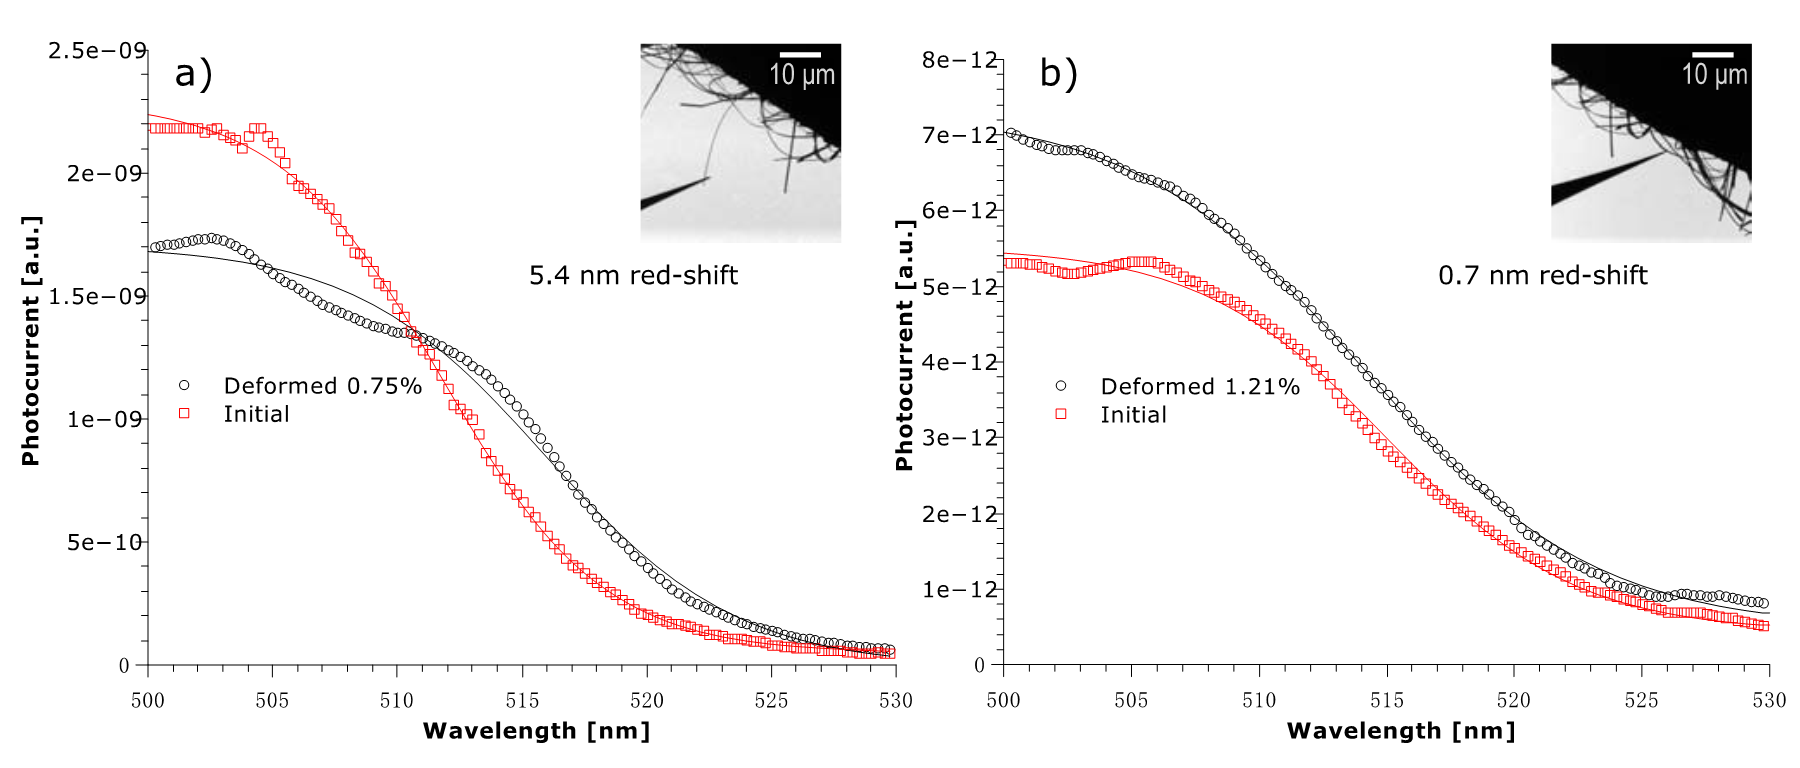
\includegraphics[width=\textwidth]{figures/figure6_s3}
\caption[Photocurrent spectroscopy of deformed CdS NW]
{(a,b) Additional examples of photocurrent spectroscopy of individual CdS nanowires, in their initial and deformed states. Low magnification TEM images are shown in the insets for each case. Strain and red-shift values are marked on each of the plots. 
\label{fig:6_s3}}
\end{figure}


Evidence of the deformation effects which could have induced the valence band decrease can be found in the HRTEM images. Figure \ref{fig:6_5} shows an image of a typical bent CdS nanowire. The diameter was measured to be around 35.6 nm, and its bending radius was 1040.7 nm, leading to a strain of 2.42\%.  Figure \ref{fig:6_5}a is a high-resolution image taken from the area marked in Figure \ref{fig:6_5}b. The result of geometric phase analysis (GPA) performed on this high-resolution image is given in Figure \ref{fig:6_5}c; the data shows that the upper-left corner of the image, oriented towards the center of the nanowire, experiences more strain than the edge region of the nanowire, located in the lower-right corner of the same image. The same GPA analysis procedure allows us to infer the locations of several defects in this area, based on abrupt changes in the calculated phase. Other defects are also likely to be present, as indicated by several regions of different contrast which are visible in the same image. It should be noted that the present nanowires were deformed elastically, compared to the previous examples where they had undergone larger strains (>10\%).\cite{Wang2013}
It should be noted that the averaged results presented here cannot accurately describe any single selected nanowire in terms of performance. The nanowires vary in regards to their morphology and structural properties, even within the same batch. There is an inherent contradiction between the need to accurately control the properties of every nanowire and the high-yield production required for making multiple devices at an industrial scale. From a statistical point of view, within this variety of structures, the nanowires studied here share common features with respect to their photocurrent-to-dark current ratio behavior during the deformation cycles. This is particularly advantageous for devices manufactured from a large amount of nanowires. Indeed, successful examples of making flexible transparent electrodes,\cite{Liu2014a} flexible photodetectors,\cite{Xu2015b} flexible supercapacitor electrodes,\cite{Liu2014a} lithium-ion batteries,\cite{Wang2015} LED arrays,\cite{Wang2015a} solar cells,\cite{Zhang2012}. out of these structures have already been reported.\\

\begin{figure}  
\centering
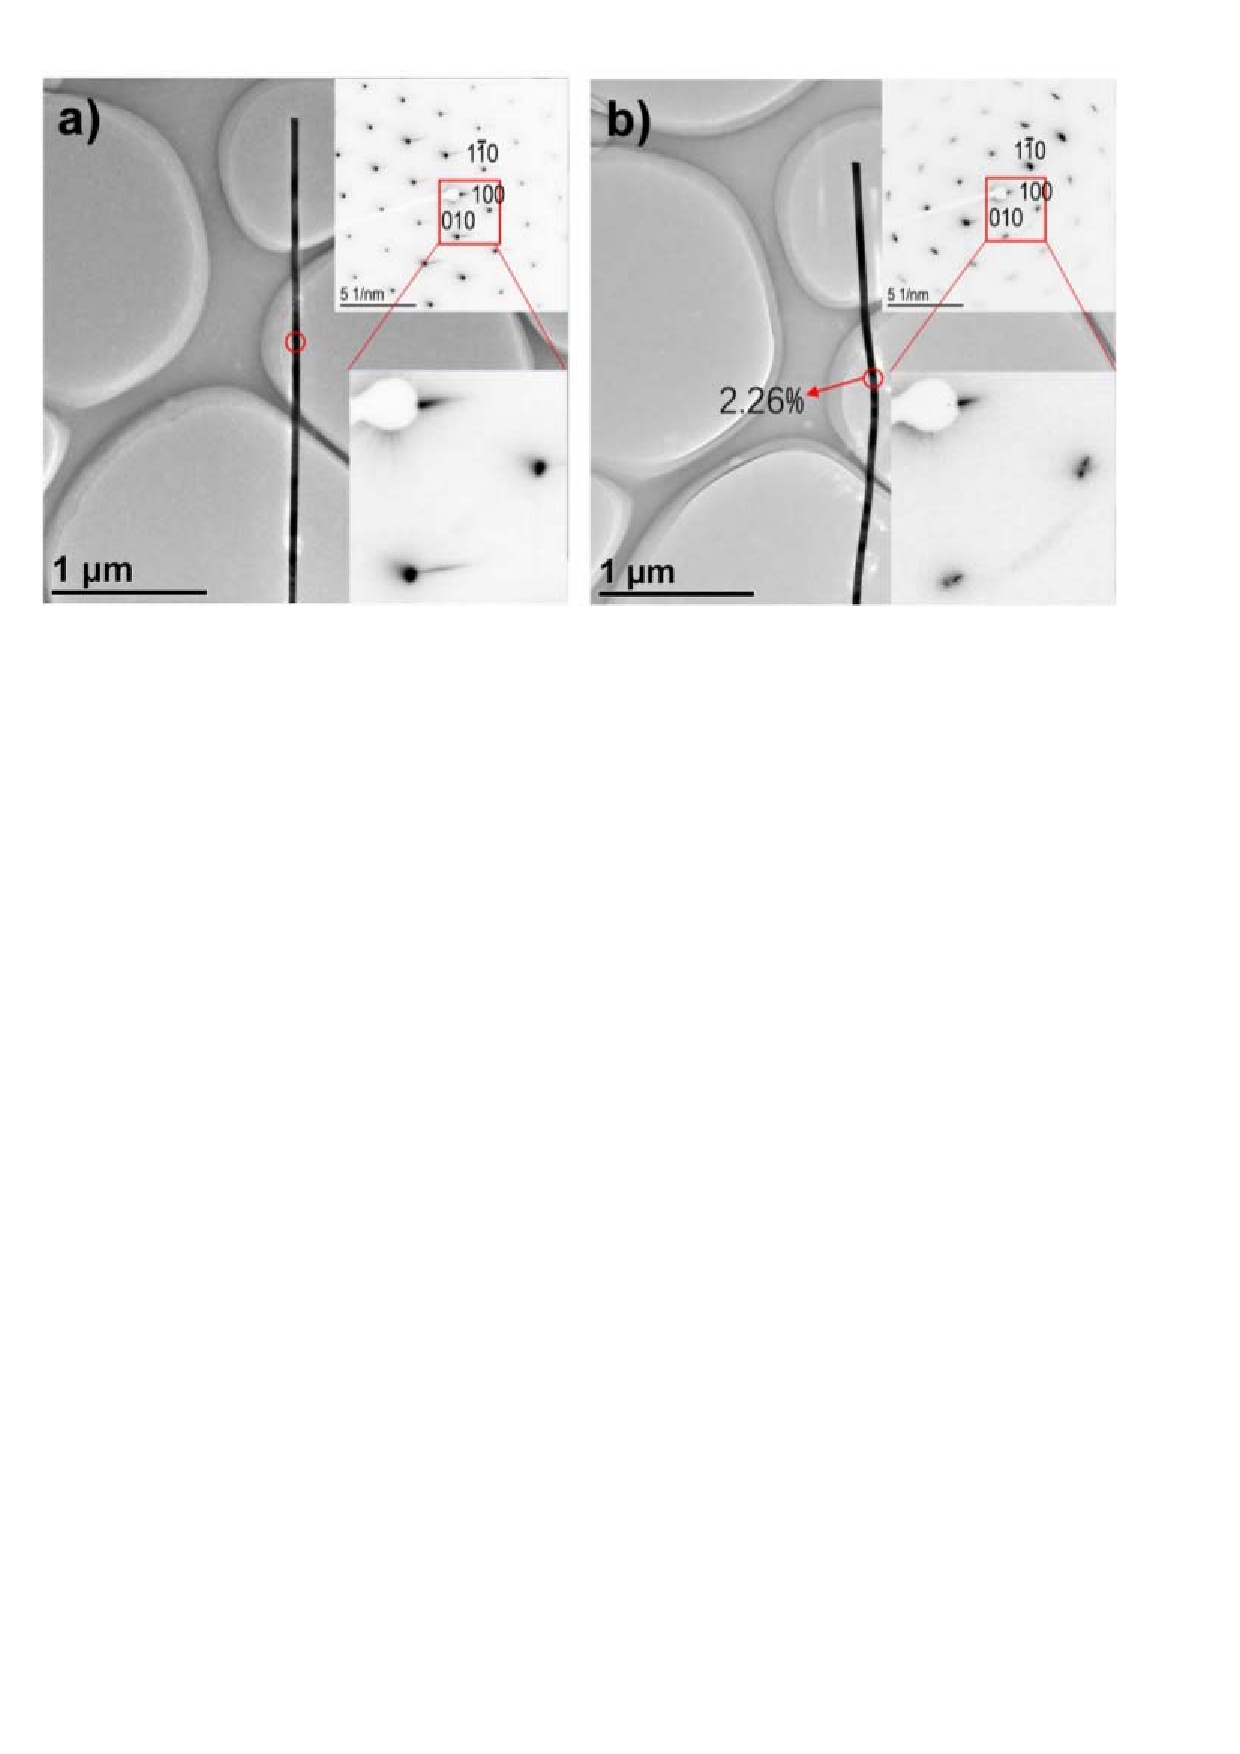
\includegraphics[width=250pt]{figures/figure6_5}
\caption[Diffraction of NW under strain]
{(a,b) TEM images of the nanowire before/after bending on a TEM carbon grid using a standard double-tilt holder due to the electron beam irradiation of the supporting C segments. The insets show SAED patterns along the [001] direction from areas marked by red circles. Representative framed parts of the SAED patterns are zoomed-in in the lower-right parts of the panels.
\label{fig:6_5}}
\end{figure}

\section{Conclusion}
To summarize, we have successfully performed pioneering photocurrent measurements for elastically deformed CdS nanowires inside the HRTEM. Using in situ electrical probing and light illumination, we have characterized the electronic (dark, light-off) and optoelectronic (light-on) features of individual nanowires undergoing mechanical deformation. To make the data reliable in a view of future technological applications, a large variety of nanowires was tested, allowing for a statistical analysis of their properties. All nanostructures reveal very close photocurrent-to-dark current ratios (ON/OFF ratios) in original, bent and recovered states, with an average value of approximately 10. Photocurrent spectroscopy of several examples shows red shifts of the order of several nanometers for the photocurrent cut-off wavelength. These small shifts are likely caused by deformation, which induces variations in the band structure. By taking HRTEM images, non-uniformly distributed lattice defects were found after bending. Our experiments reveal a variety of bending-induced effects for individual nanowires, while showing that from a statistical point of view the nanowires display common features in their response to deformation, making them suitable for future flexible optoelectronic applications. 

